
\documentclass[46pt, nnermargin=7mm, blockverticalspace=7mm, colspace=7mm]{tikzposter}\usepackage[]{graphicx}\usepackage[]{color}
%% maxwidth is the original width if it is less than linewidth
%% otherwise use linewidth (to make sure the graphics do not exceed the margin)
\makeatletter
\def\maxwidth{ %
  \ifdim\Gin@nat@width>\linewidth
    \linewidth
  \else
    \Gin@nat@width
  \fi
}
\makeatother

\definecolor{fgcolor}{rgb}{0.345, 0.345, 0.345}
\newcommand{\hlnum}[1]{\textcolor[rgb]{0.686,0.059,0.569}{#1}}%
\newcommand{\hlstr}[1]{\textcolor[rgb]{0.192,0.494,0.8}{#1}}%
\newcommand{\hlcom}[1]{\textcolor[rgb]{0.678,0.584,0.686}{\textit{#1}}}%
\newcommand{\hlopt}[1]{\textcolor[rgb]{0,0,0}{#1}}%
\newcommand{\hlstd}[1]{\textcolor[rgb]{0.345,0.345,0.345}{#1}}%
\newcommand{\hlkwa}[1]{\textcolor[rgb]{0.161,0.373,0.58}{\textbf{#1}}}%
\newcommand{\hlkwb}[1]{\textcolor[rgb]{0.69,0.353,0.396}{#1}}%
\newcommand{\hlkwc}[1]{\textcolor[rgb]{0.333,0.667,0.333}{#1}}%
\newcommand{\hlkwd}[1]{\textcolor[rgb]{0.737,0.353,0.396}{\textbf{#1}}}%

\usepackage{framed}
\makeatletter
\newenvironment{kframe}{%
 \def\at@end@of@kframe{}%
 \ifinner\ifhmode%
  \def\at@end@of@kframe{\end{minipage}}%
  \begin{minipage}{\columnwidth}%
 \fi\fi%
 \def\FrameCommand##1{\hskip\@totalleftmargin \hskip-\fboxsep
 \colorbox{shadecolor}{##1}\hskip-\fboxsep
     % There is no \\@totalrightmargin, so:
     \hskip-\linewidth \hskip-\@totalleftmargin \hskip\columnwidth}%
 \MakeFramed {\advance\hsize-\width
   \@totalleftmargin\z@ \linewidth\hsize
   \@setminipage}}%
 {\par\unskip\endMakeFramed%
 \at@end@of@kframe}
\makeatother

\definecolor{shadecolor}{rgb}{.97, .97, .97}
\definecolor{messagecolor}{rgb}{0, 0, 0}
\definecolor{warningcolor}{rgb}{1, 0, 1}
\definecolor{errorcolor}{rgb}{1, 0, 0}
\newenvironment{knitrout}{}{} % an empty environment to be redefined in TeX

\usepackage{alltt} % See Section 3

% Use fancy fonts
\usepackage{fontspec}
\setmainfont{Liberation Sans}
\setsansfont{SourceSansPro-Regular}
\setmonofont{Consolas}

\usepackage{hyperref}
\hypersetup{
  colorlinks=true,
  linkcolor=black,
  citecolor=black,
  filecolor=black,
  urlcolor=blue
}
\urlstyle{sf}

% can use captions outside figure environments
\usepackage{capt-of}

% Latex special characters are rendered correctly with XeTeX
\usepackage{xltxtra}
\usepackage{xunicode}
\defaultfontfeatures{Mapping=tex-text}

\title{\textbf{Using iNaturalist to engage the public and learn more about echinoderms}}

\institute{Florida Museum of Natural History, University of Florida,
  Gainesville, FL 32611 \\
  \vspace{1cm}
  {\normalsize francois.michonneau@gmail.com, paulay@flmnh.ufl.edu} }

\author{Fran\c{c}ois Michonneau, Gustav Paulay}


\usetheme{Autumn}
\IfFileExists{upquote.sty}{\usepackage{upquote}}{}
\begin{document}





\maketitle

%----------------------      poster starts here    ----------------------------%

\begin{columns}

\column{.43}
\block{Introduction}{

  Echinoderms are among the most conspicuous and abundant marine
  invertebrates. Several species of echinoderms undergo important demographic
  fluctuations for reasons that are not always well understood (e.g.,
  crown-of-thorns outbreaks, \textit{Diadema antillarum} die-off,
  starfish-wasting-syndrome), with important ecological consequences. In
  addition, many species are targeted by unregulated fisheries.
  
  \vspace{.5cm}

  Despite these factors, echinoderms have not received a lot of taxonomic
  attention, and many large species remain undescribed and/or poorly
  known. Regularly, field guides illustrate undescribed species, and divers
  commonly photograph new or poorly known species.
  
  \vspace{.5cm}

  With recent technological advances, it has become increasingly easier to
  document species encountered in nature. For instance, smartphones can, with
  the single touch of the screen, take a picture while associating the exact
  geographical location and time of the observation. Digital cameras have made
  underwater photography much more accessible, and many divers now document the
  species they encounter by sharing their pictures on social media websites.

  \vspace{.5cm}

  Our knowledge of echinoderms could therefore be improved by aggregating user
  observations of these organisms, while educating the public at the same time
  about these fascinating organisms.

  }

\column{.57}
\block{What is iNaturalist?}{ 

  iNaturalist (\href{http://inaturalist.org}{http://inaturalist.org}) is a
  website that allows users to submit observations about any species, along with
  images, GPS coordinates and ancillary information about the habitat or natural
  history. Once submitted the observations can be further identified by the
  community and validated by "curators". This mechanism allows users to hone
  their identification skills, learn about the organisms, and communicate with
  each other. Observations in turn provide a wealth of information about
  distribution, variation, abundance, and other aspects of natural history.

  \vspace{.5cm}

  We started a project on Echinoderms
  (\href{http://inaturalist.org/projects/echinoderms}{http://inaturalist.org/projects/echinoderms})
  to gather observations worldwide, and across taxa. Our goal is to improve our
  knowledge of species distributions, variation, and biology, and to educate the
  public about the diversity of Echinoderms. This platform provides a great
  outreach tool facilitating communication between scientists and
  naturalists. Because iNaturalist is easy to use and has applications for
  mobile devices, it can also be used during organized citizen science
  initiatives such as Bioblitz, or class field trips.

  \vspace{.5cm}

  This crowd-sourcing effort has the potential to greatly facilitate the
  documentation of species diversity, occurrences, variation, changes in
  distributions and species density (e.g., crown-of-thorns outbreaks,
  consequences of the starfish wasting syndrome) while educating the public
  about echinoderms

  \vspace{.5cm}

  Over a hundred users have already contributed 700+ observations. We will
  advertise the project more widely to the SCUBA diving community and through
  citizen science initiatives. We welcome everyone to submit observations or
  help curating the observations submitted to the project. Don't hesitate to
  join us!

}

\end{columns}


\begin{columns}

\column{0.25}
\block{Project page}{

\begin{center}
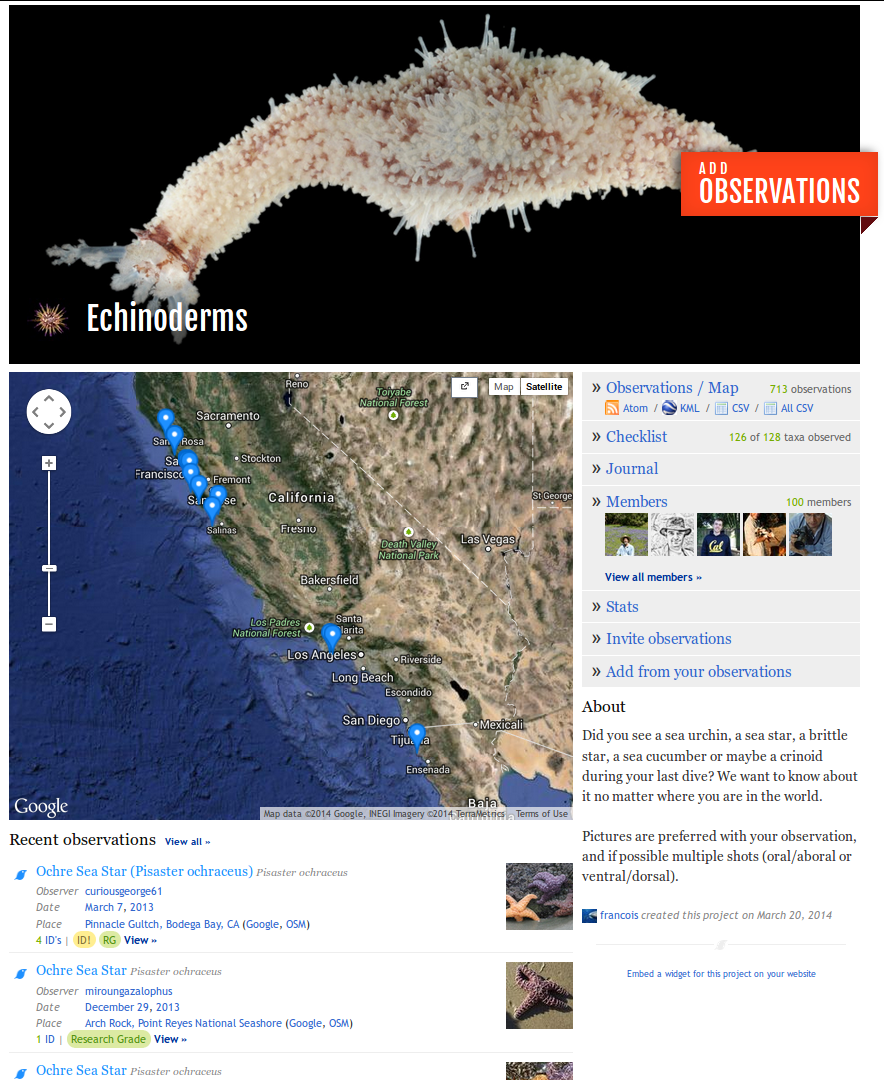
\includegraphics[width=.215\columnwidth]{images/inat-echino}
\captionof{figure}{The Echinoderm project on iNaturalist}
\end{center}

}

\column{0.25}
\block{User observation}{

\begin{center}
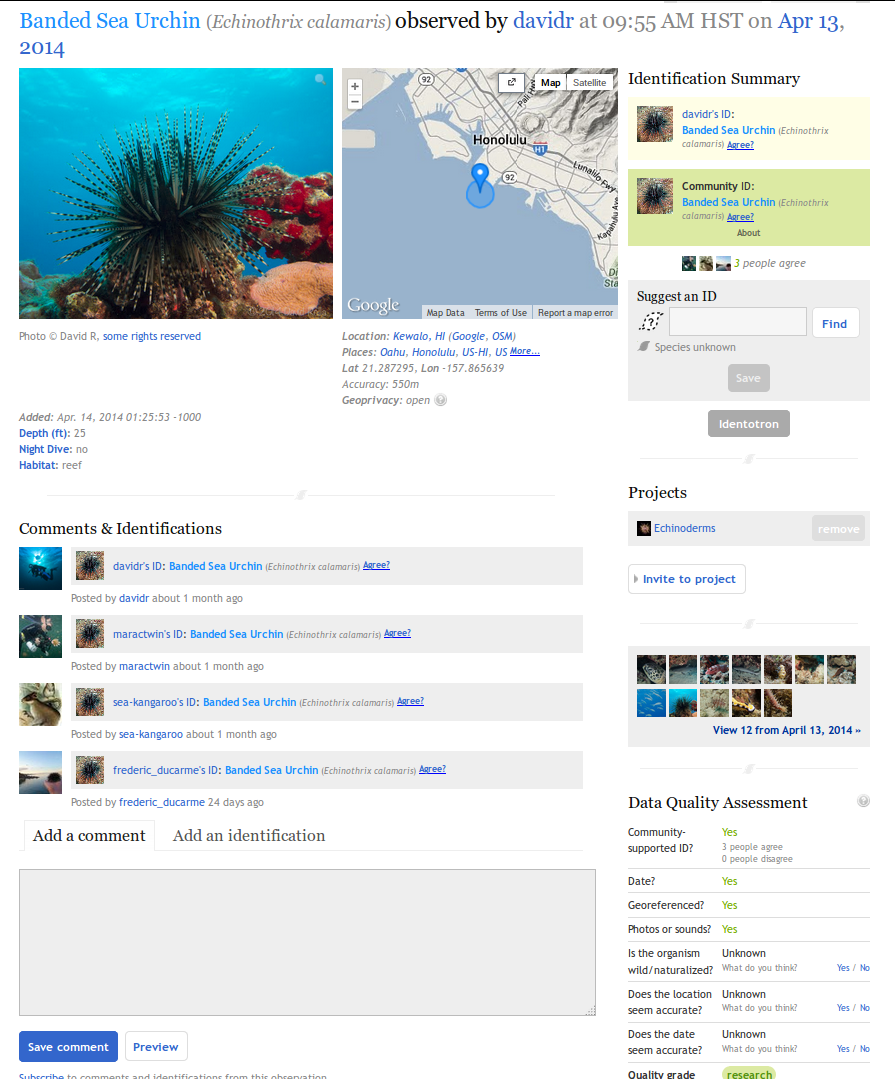
\includegraphics[width=.215\columnwidth]{images/inat-screenshot}
\captionof{figure}{Example of an user-submitted observation}
\end{center}

}

\column{0.25}
\block{Observations per class}{

\begin{center}
\begin{knitrout}
\definecolor{shadecolor}{rgb}{0.969, 0.969, 0.969}\color{fgcolor}
\includegraphics[width=.22\columnwidth]{figures/latex-abundance-per-class} 

\end{knitrout}
\captionof{figure}{Number of observations per class}
\end{center}

\vspace{.8cm}

Large and abundant species from the intertidal of the Western United States
dominate the observations at present, reflecting the development of iNaturalist
in California. However, underwater sightings from the Caribbean and the
Indo-West Pacific also represent a large proportion of the observations.
}

\column{0.25}
\block{Most recorded species}{
\begin{center}
\begin{knitrout}
\definecolor{shadecolor}{rgb}{0.969, 0.969, 0.969}\color{fgcolor}
\includegraphics[width=.212\columnwidth]{figures/latex-top-species} 

\end{knitrout}
\captionof{figure}{List of the 20 species the most observed on iNaturalist}
\end{center}
}



\end{columns}

% --- start map

\begin{columns}

\column{.7}
\block{Map of recorded observations}{

\begin{center}
\begin{knitrout}
\definecolor{shadecolor}{rgb}{0.969, 0.969, 0.969}\color{fgcolor}
\includegraphics[width=.67\columnwidth]{figures/latex-all-observations} 

\end{knitrout}
\captionof{figure}{Global distribution of observations recorded by iNaturalist users} 
\end{center}

}

\column{.3}
\block{Distribution maps}{

\begin{center}
\begin{knitrout}
\definecolor{shadecolor}{rgb}{0.969, 0.969, 0.969}\color{fgcolor}
\includegraphics[width=.255\columnwidth]{figures/latex-map-pisaster-strongylo} 

\end{knitrout}
\captionof{figure}{Distribution map for two highly observed species generated
  from user observations}
\end{center}

\vspace{2mm}

}
\end{columns}

% --- end maps

% --- footer

\block{}{

  {\small This poster is open-source (CC-BY), fully reproducible and available
    on Figshare (DOI:
    \href{http://dx.doi.org/10.6084/m9.figshare.1040435}{10.6084/m9.figshare.1040435}). The
    source code can be obtained from:
    \href{https://github.com/fmichonneau/inat-poster/}{http://github.com/fmichonneau/inat-poster}. It
    was made possible using the LaTeX package
    \href{http://www.ctan.org/pkg/tikzposter}{tikzposter}, and
    \href{http://www.r-project.org}{R} complemented with the packages
    \href{https://github.com/hadley/ggplot2/}{ggplot2} (by Hadley Wickham),
    \href{http://yihui.name/knitr/}{knitr} (by Yihui Xie),
    \href{http://f1000research.com/articles/2-191/v2}{taxize} (by Scott
    Chamberlain \& Eduard Szocs), and
    \href{https://github.com/karthik/wesanderson}{wesanderson} (by Karthik Ram).
  }

} 
% ---- end footer

\end{document}
